% This table is used in overview.tex, but because it spans multiple columns we have to declare it further up to convince LaTeX to place it near the text that references it.
\begin{table*}[htbp]
\caption{
Visualization algorithms accelerated by VTK-m.
}
\label{tab:algorithms}
\begin{tabularx}{\textwidth}{lX}
\toprule
    Goals of visualization & Algorithms accelerated by VTK-m\\
    \midrule
    Scalar field visualization & Contour \cite{Lo2012}, Threshold \cite{Maynard2013}  \\
    Vector/Flow field visualization & Particle advection~\cite{Pugmire2018}, Finite-time Lyapunov exponent (FTLE) \cite{Sane2021:EGPGV}, Poincar\'{e} plot~\cite{Suchyta2022}  \\
    Geometry Refinement & External faces \cite{Lessley2016,Lessley2017}, Surface simplification \cite{Moreland2016}, Point merging \cite{Yenpure2019} \\
    Rendering & Volume rendering \cite{Larsen2015:VR}, Surface rendering \cite{Larsen2015:RayTrace}  \\
    Reduction and compression &
    Wavelet compression \cite{Li2017}, Statistical models \cite{Wang2019},  Lagrangian Representations \cite{Sane2021:ICCS,Sane2021:EGPGV}  \\
    Topological analysis & Contour trees \cite{Carr2021}  \\
    Uncertainty visualization & Uncertainty isosurface \cite{Wang2023}  \\
\bottomrule
\end{tabularx}
\end{table*}



% This figure is used in overview.tex, but because it spans multiple columns we have to declare it further up to convince LaTeX to place it near the text that references it.
\begin{figure*}[tb]
  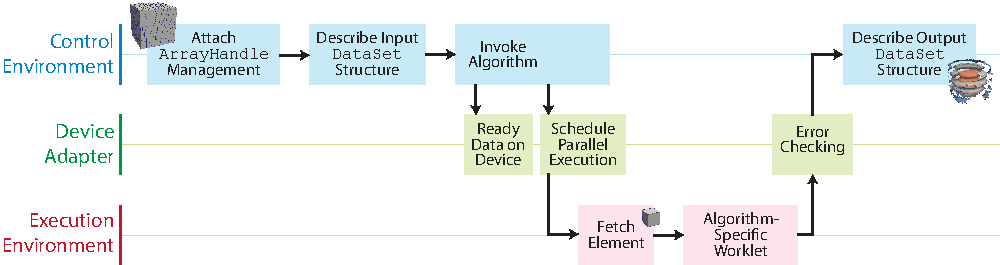
\includegraphics[width=\textwidth]{vtkm-workflow}
  \caption{
    Workflow of an algorithm implemented in \vtkm.
    The ``control environment,'' which runs on a single thread on the host, manages data organization and orchestrates operations.
    The ``execution environment,'' which runs on many threads on the device, performs parallel execution across elements of data.
    A ``device adapter'' manages data movement and control flow between these two environments.
  }
  \label{fig:vtkm-workflow}
\end{figure*}


\section{Introduction}

%\ken{Do not add OverLeaf comments to this document. They will not be seen! Instead, use the comment command with your name to add the comment to the text. We'll see the comment when reviewing the paper. The commands are defined near the top of IJHPCASpecialIssue\_VTKm.tex.}

%\ken{Please complete your writing assignments by January 22.}

%\assign{Hank, do an editing pass.}

%The Exascale Computing Project (ECP) brought high-performance computing to the next milestone of capacity computing.\hank{I do not understand the preceding sentence.  Capability?  And we already had HPC.  How did ECP bring HPC?}
As its name would imply, the goal of the Exascale Computing Project (ECP) was to build and make practical the world's first exascale supercomputers.
Although this goal was nominally to stand up computers capable of a billion-billion ($10^{18}$) floating point operations per second, this advancement required a revolution in both hardware and software.
Critical to this advancement was the adoption of GPUs (from a variety of vendors) to be used as the primary computing engine.
These GPUs provided unmatched computational throughput relative to the power they consume, albeit at the cost of greater code complexity.%
\blfootnote{Notice: This manuscript has been authored by UT-Battelle LLC under contract DE-AC05-00OR22725 with the US Department of Energy (DOE). The US government retains and the publisher, by accepting the article for publication, acknowledges that the US government retains a nonexclusive, paid-up, irrevocable, worldwide license to publish or reproduce the published form of this manuscript, or allow others to do so, for US government purposes. DOE will provide public access to these results of federally sponsored research in accordance with the DOE Public Access Plan (\url{https://www.energy.gov/doe-public-access-plan}).}

Scientific simulations running on exascale supercomputers can produce datasets of unprecedented
scale, and
visualization and analysis approaches are frequently used to understand the resulting
data and promote discovery.
%
That said, the scale of the data produced by simulations on exascale computers requires
the visualization and analysis approaches themselves to utilize significant computational resources.
%
Most commonly, this computation is conducted on the same supercomputer and hardware that produced
the data in the first place.

The \vtkm software library makes it possible to process these enormous datasets from exascale computers
by implementing classic scientific visualization algorithms that have been redesigned for heavily threaded environments such as supercomputers with GPUs.
\vtkm also provides a framework that simplifies the implementation of new algorithms and adds a porting layer to work across multiple processor types.
This porting layer allows algorithms written in \vtkm to be written once and run everywhere, which alone saves a substantial amount of developer effort.
At the inception of the ECP, \vtkm was the byproduct of a research project.
The ECP provided the investment to advance \vtkm to production software.
This software now serves as the underlying visualization implementation across the entire ECP.
\vtkm is currently used by ParaView, VisIt, and Ascent for the portion of their visualization algorithms that execute on the accelerator processors of exascale platforms and on other GPU-centric supercomputers.

This paper describes the challenges encountered when making visualization available at exascale.
It begins with a brief overview of the \vtkm framework.
It then describes the most significant porting challenges encountered during the ECP given the hardware for the production exascale machines differed dramatically from the pre-exascale machines.
This is followed by a summary of the performance of \vtkm on the exascale hardware including scaling studies on an exascale computer of over 37,000 AMD GPUs.
Finally, the paper concludes with a discussion on the software engineering required to integrate \vtkm into usable visualization tools and successes with using \vtkm to solve problems in real science applications.
This includes porting challenges, performance testing and improvement, integration with other ECP software technologies, and the support of ECP applications.
